\subsection{Estimation of Drell-Yan and diboson backgrounds}
\label{sec:DY_diboson}

The background from Drell-Yan (DY) events is strongly reduced by our event selection which applies several cuts on \met-related variables.
In this section, we discuss these cuts and the properties of the DY background in more detail using a  
control region defined by a 0 b-jet requirement and an on-Z requirement defined by $|m_{ll} - m_Z| < 15$ GeV.

Figure~\ref{fig:DY} shows the distributions of \metSig and \mtll  for same-flavour ($ee$/$\mu\mu$) events in this control region, 
before applying the $\metSig>5$ cut. Because \met in DY events typically arises from jet mismeasurements, large \met will be countered by large \HT, and hence
the \metSig distribution peaks below 5 for the DY background.  
Backgrounds with genuine \ETmiss (and the signal) are typically concentrated at higher~\metSig.

When \met originates from jet mismeasurements, it is also likely to align with one of the jets, which is exploited by the cuts on the $\cos{\Delta\phi(\met, \text{jet})}$ variables that are shown in Fig.~\ref{fig:DY_afterMetSig} for the two leading jets and after applying the $\metSig>5$ cut. 
It can readily be seen that this selection is dominated by a mixture of DY and multiboson contributions that we now separate. 
In DY events, the \ETmiss will be dominated by mismeasurement of jets. 
If we therefore veto events where one of the two leading jets is aligned with \ETmiss according to $\cos{\Delta\phi(\met, \text{leading jet})} > 0.8$ or $\cos{\Delta\phi(\met, \text{2nd leading jet})} > \cos{0.25}=0.96$, 
we can define a region where DY is pure. 
The reason for the relatively small angular separation of \ETmiss w.r.t to the sub-leading jet that it should select events with
drastic mismeasurements. Indeed, it can happen that the leading generated jet looses enough energy such that it is reconstructed as the subleading jet. 
In such cases, \ETmiss is typically aligned with the sub-leading jet to within half the jet clustering distance.

In Fig.~\ref{fig:DY_dPhiInv}a, we show the \mtll distribution in this selection. The purity of DY is 84\%. 
Subtracting from data any residual electroweak contributions according to
\begin{equation}
R = \frac{n_\text{data}-n_\text{residual}}{n_\text{DY}},
\end{equation} 
we find a scale factor for DY of $1.30\pm 0.12$.

In order to justify that the scale factor is applied inclusively to the sample, we note that the \Nbtags shape is consistent with a flat scaling as shown in Fig.~\ref{fig:DY_nbtag_validation}a.
In Fig.~\ref{fig:DY_nbtag_validation}b we show the \Nbtags multiplicity after removing \mtll, \ETmiss, \metSig and $\Delta\phi$ requirements. This demonstrates the quality of \Nbtags modeling in simulated DY events. 

\begin{figure}[!hbtp]
\centering
\subfloat[\metSig]{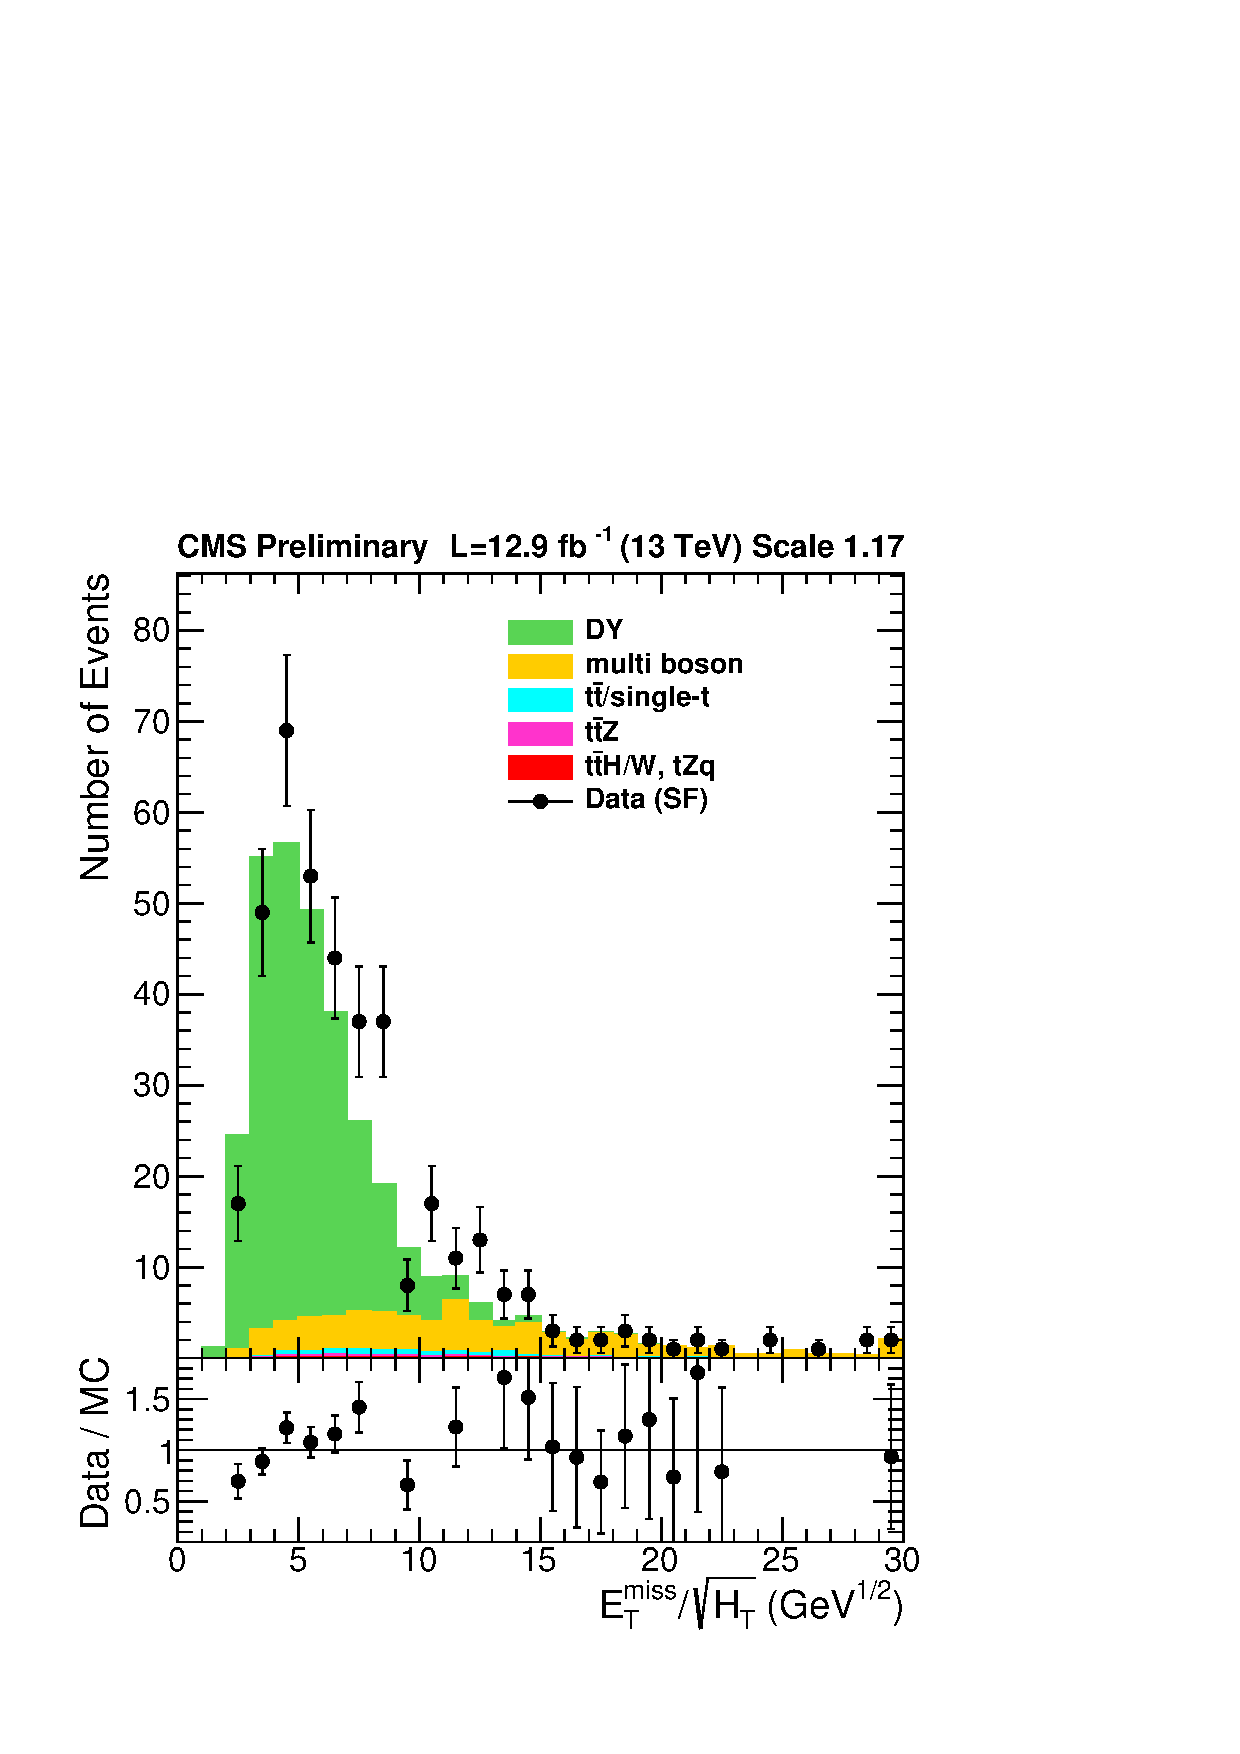
\includegraphics[width=0.45\textwidth]{figures/analysisPlots/SF/njet2-btag0-multiIsoWP-looseLeptonVeto-mll20-onZ-met80-mt2ll100/metSig.pdf}}
\subfloat[\mtll]{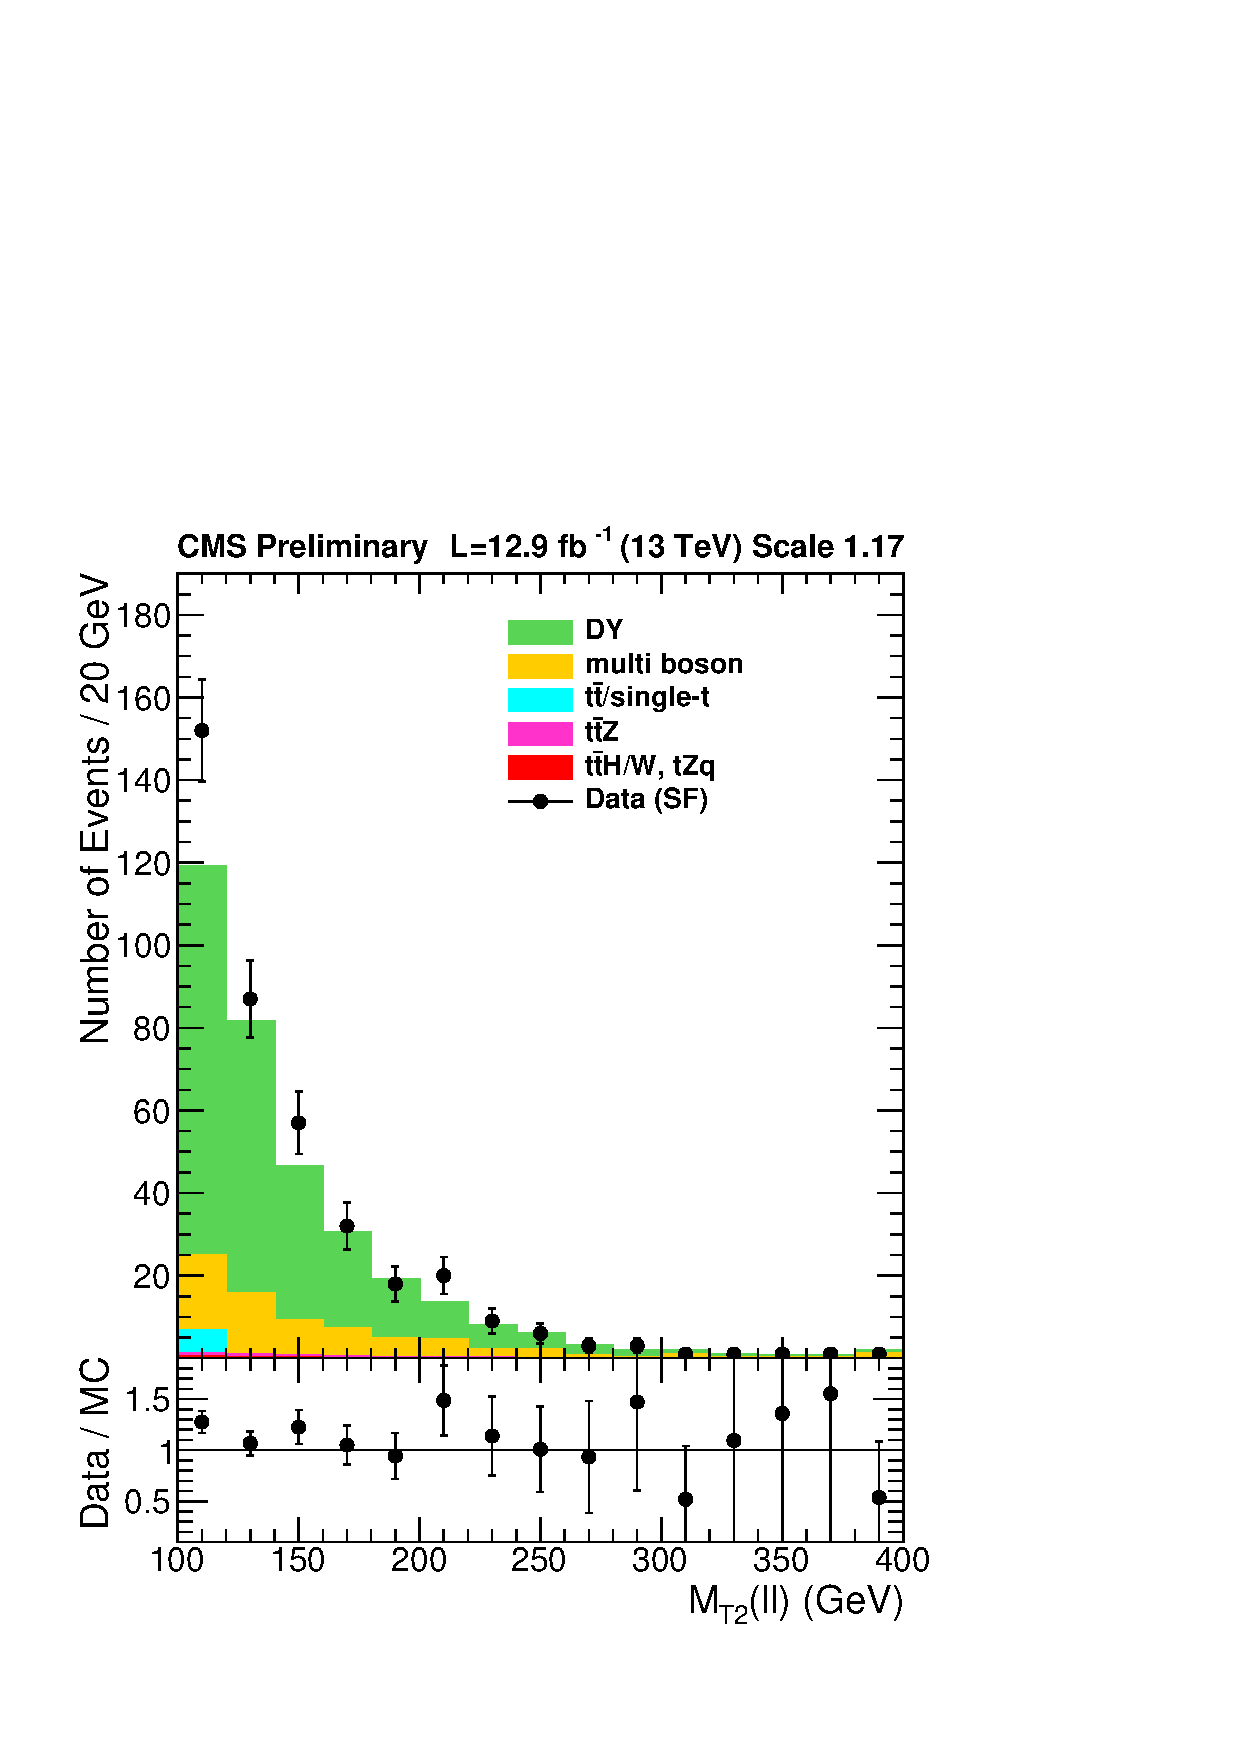
\includegraphics[width=0.45\textwidth]{figures/analysisPlots/SF/njet2-btag0-multiIsoWP-looseLeptonVeto-mll20-onZ-met80-mt2ll100/dl_mt2ll.pdf}} \\
%   \subfloat[$\cos{\Delta\phi(\met, \text{leading jet})}$]{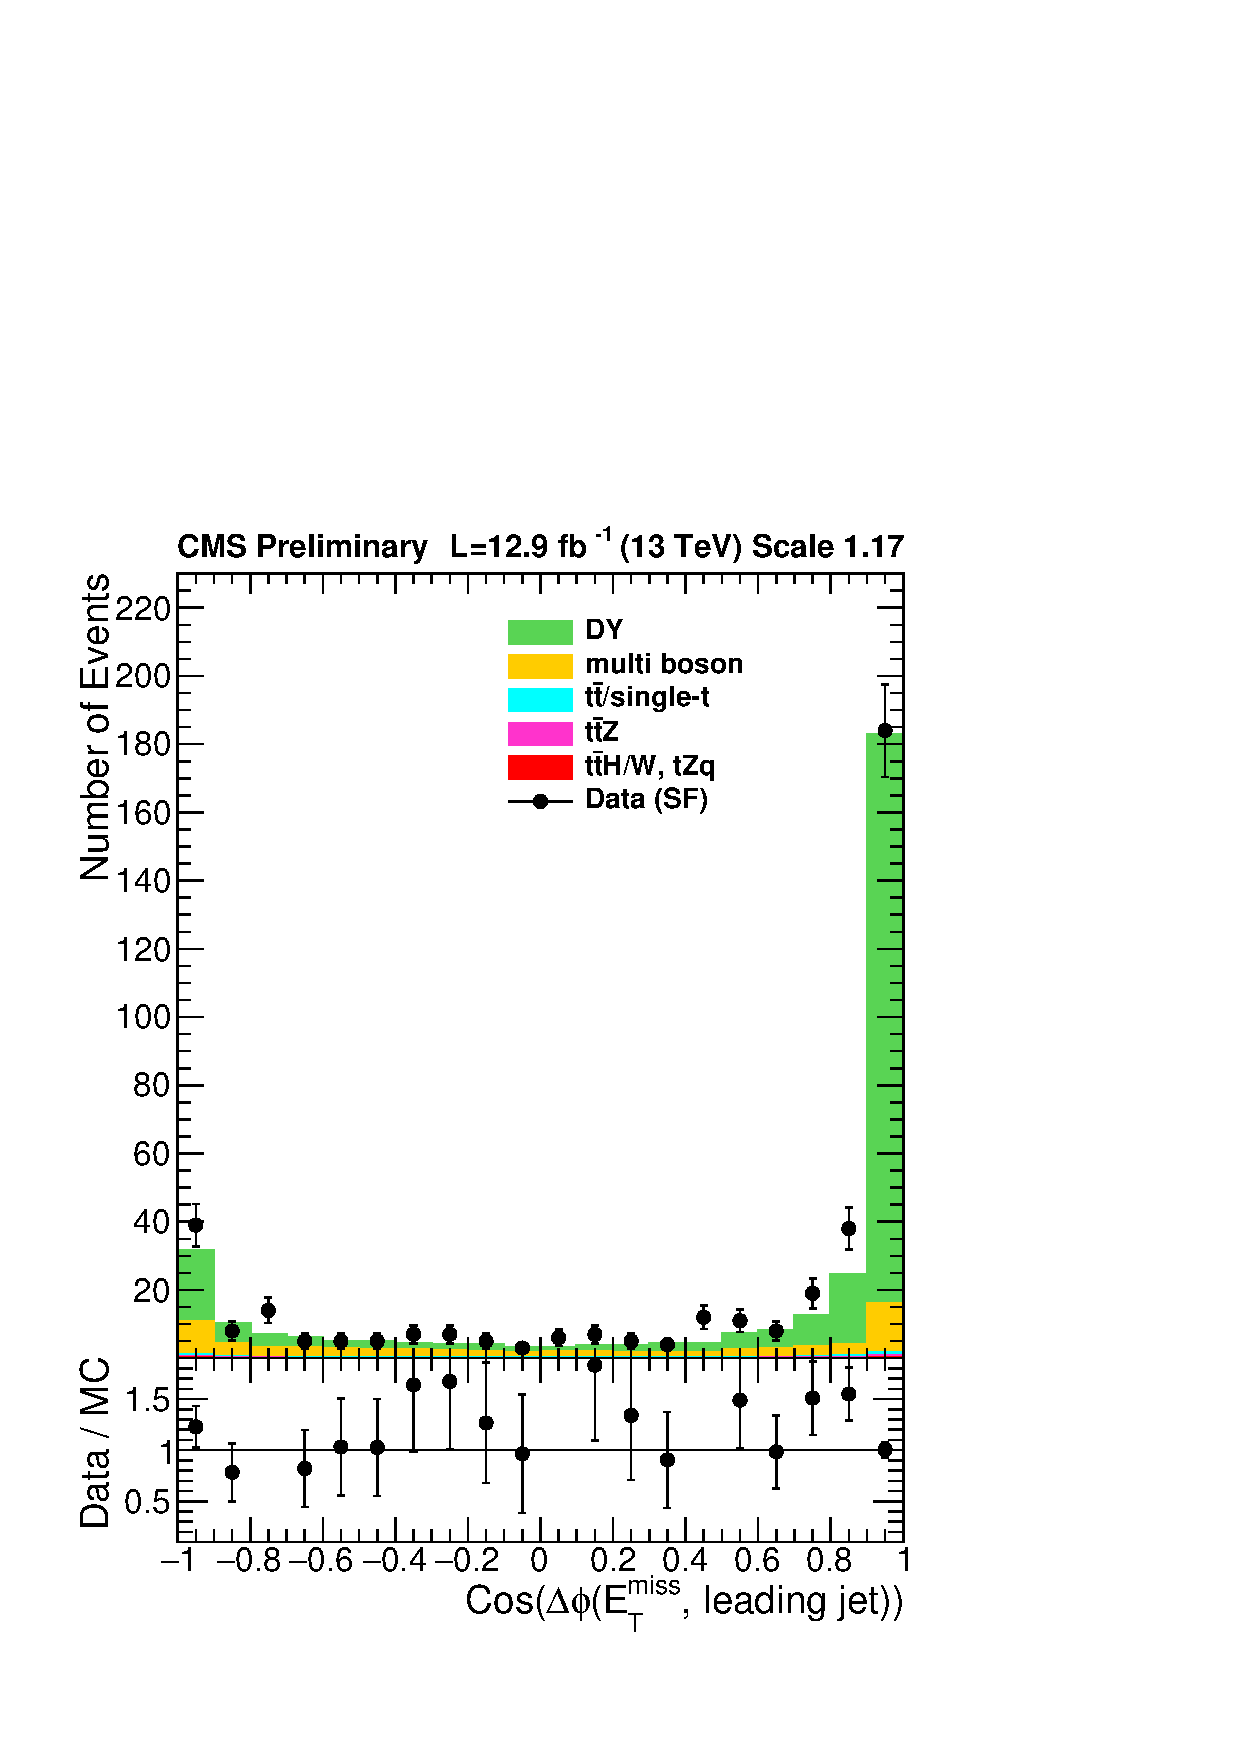
\includegraphics[width=0.45\textwidth]{figures/analysisPlots/SF/njet2-btag0-multiIsoWP-looseLeptonVeto-mll20-onZ-met80-mt2ll100/cosMetJet1phi_smallBinning.pdf}}
%   \subfloat[$\cos{\Delta\phi(\met, \text{2nd leading jet})}$]{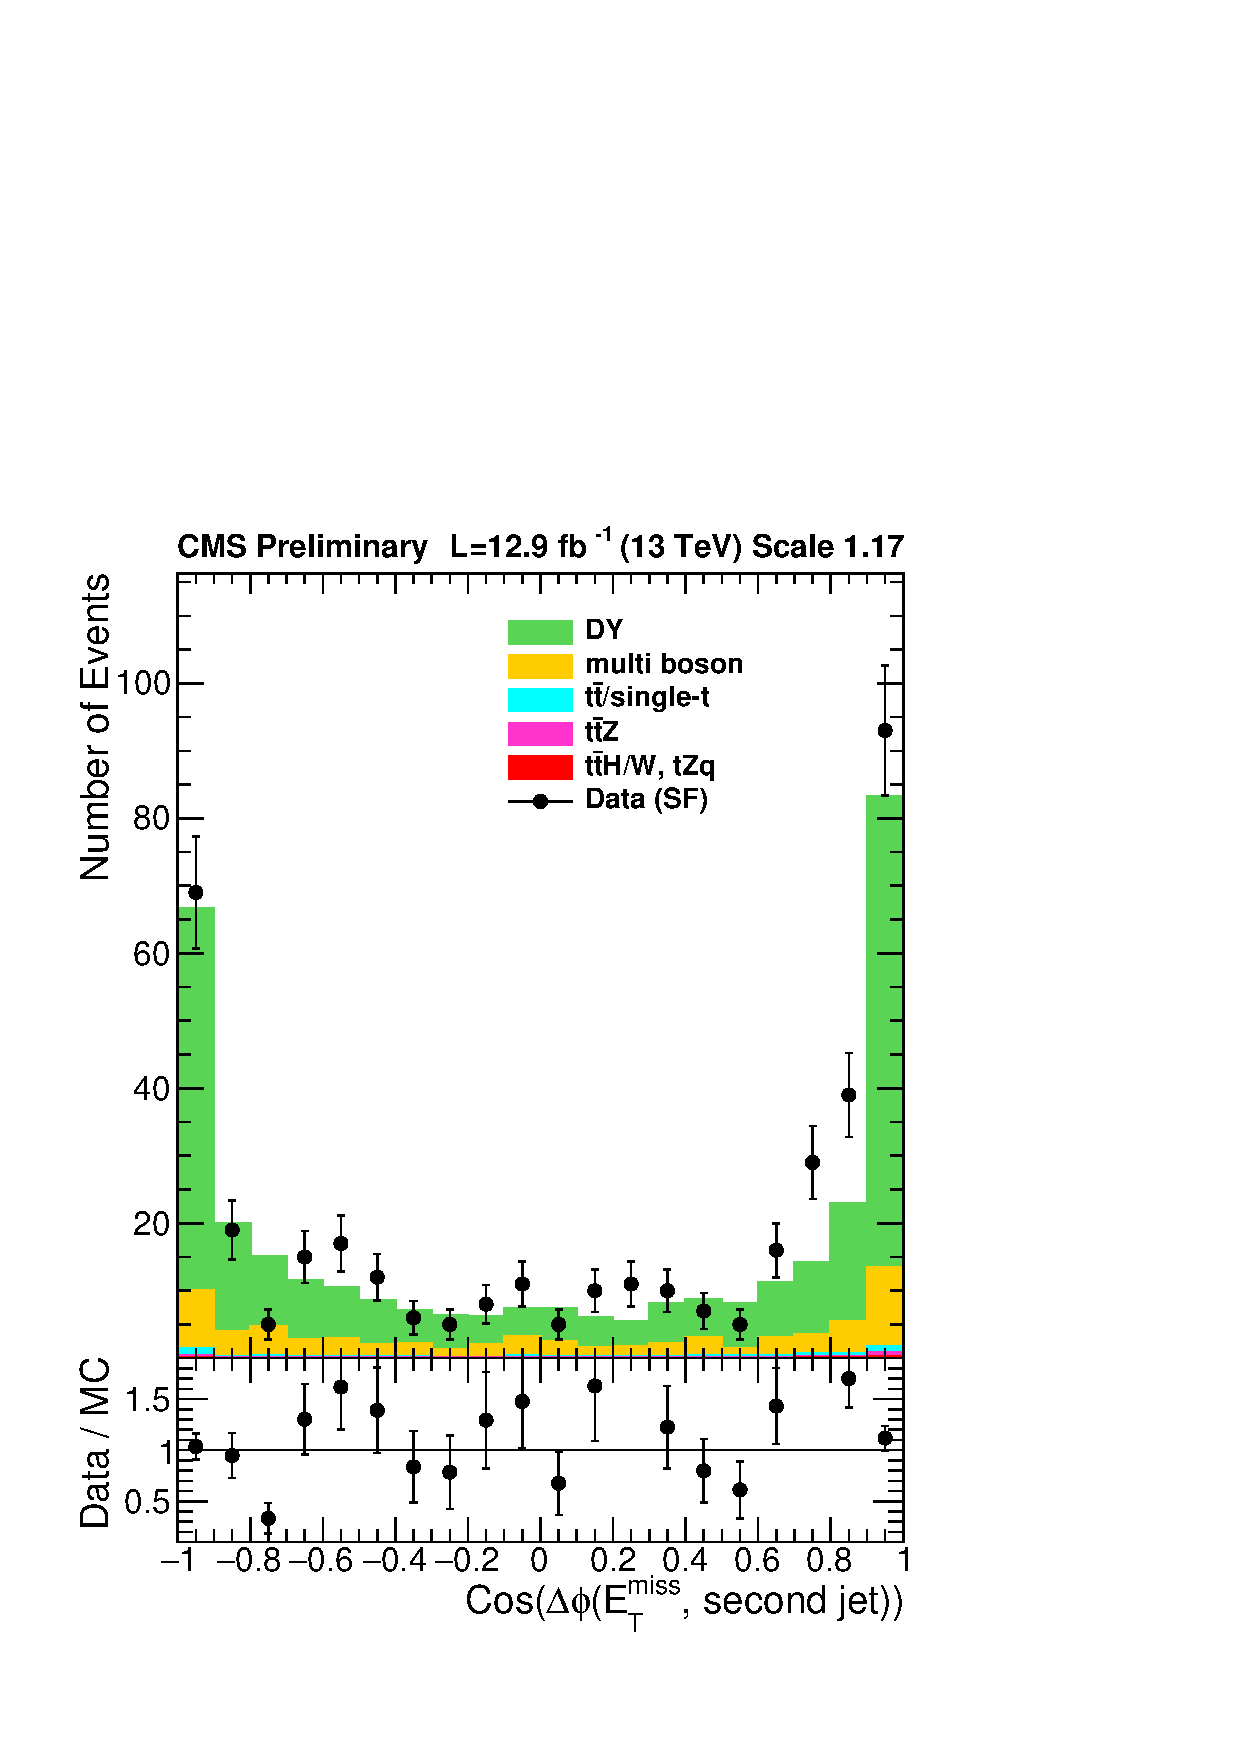
\includegraphics[width=0.45\textwidth]{figures/analysisPlots/SF/njet2-btag0-multiIsoWP-looseLeptonVeto-mll20-onZ-met80-mt2ll100/cosMetJet2phi_smallBinning.pdf}}
\caption{Distributions of \metSig, \mtll for same-flavour ($ee$/$\mu\mu$) events falling within the $Z$-mass window, with two jets and exactly 0 $b$-tags, $\met > 80$ GeV
     and $\mtll > 100$ GeV.}
\label{fig:DY}
\end{figure}

\begin{figure}[!hbtp]
\centering
\subfloat[$\cos{\Delta\phi(\met, \text{leading jet})}$]{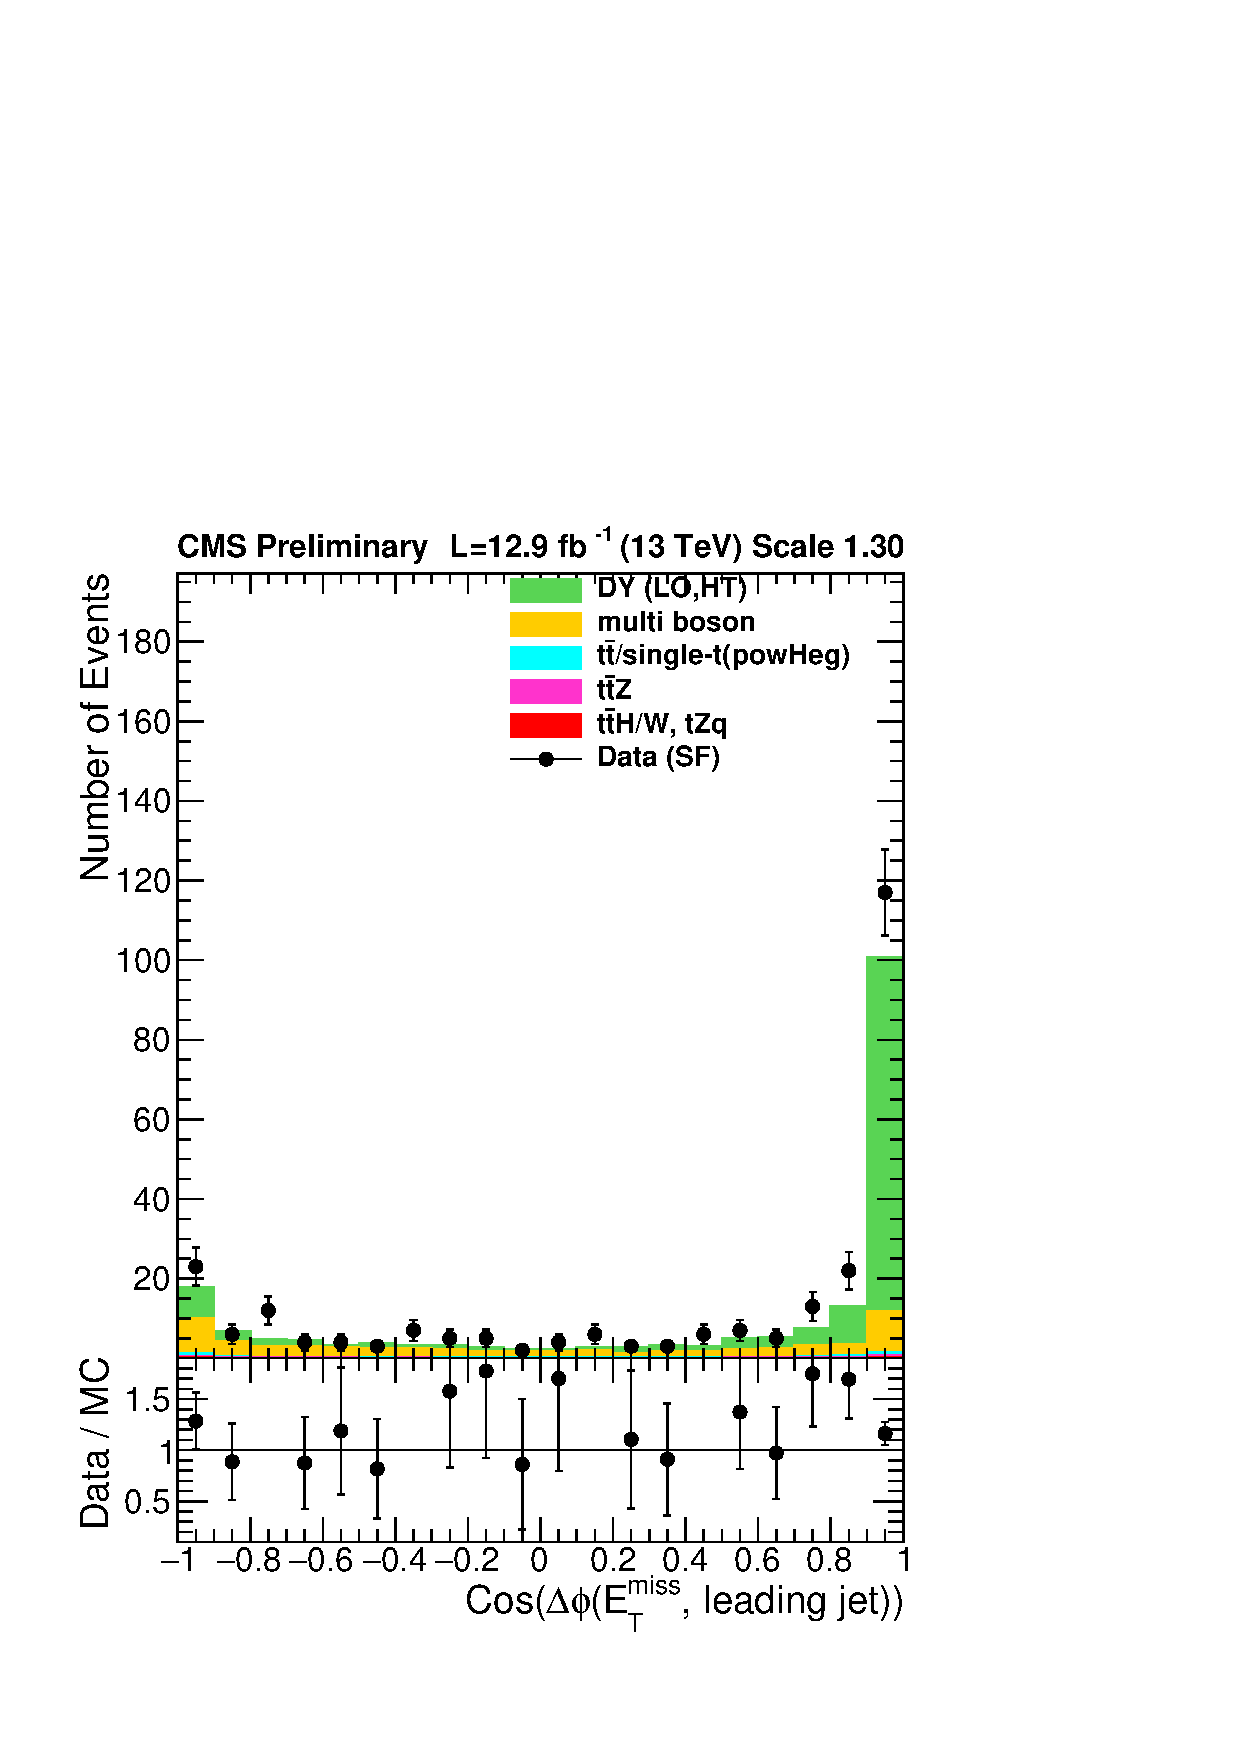
\includegraphics[width=0.4\textwidth]{figures/analysisPlots/SF/njet2-btag0-multiIsoWP-looseLeptonVeto-mll20-onZ-met80-metSig5-mt2ll100/cosMetJet1phi_smallBinning.pdf}}
\subfloat[$\cos{\Delta\phi(\met, \text{2nd leading jet})}$]{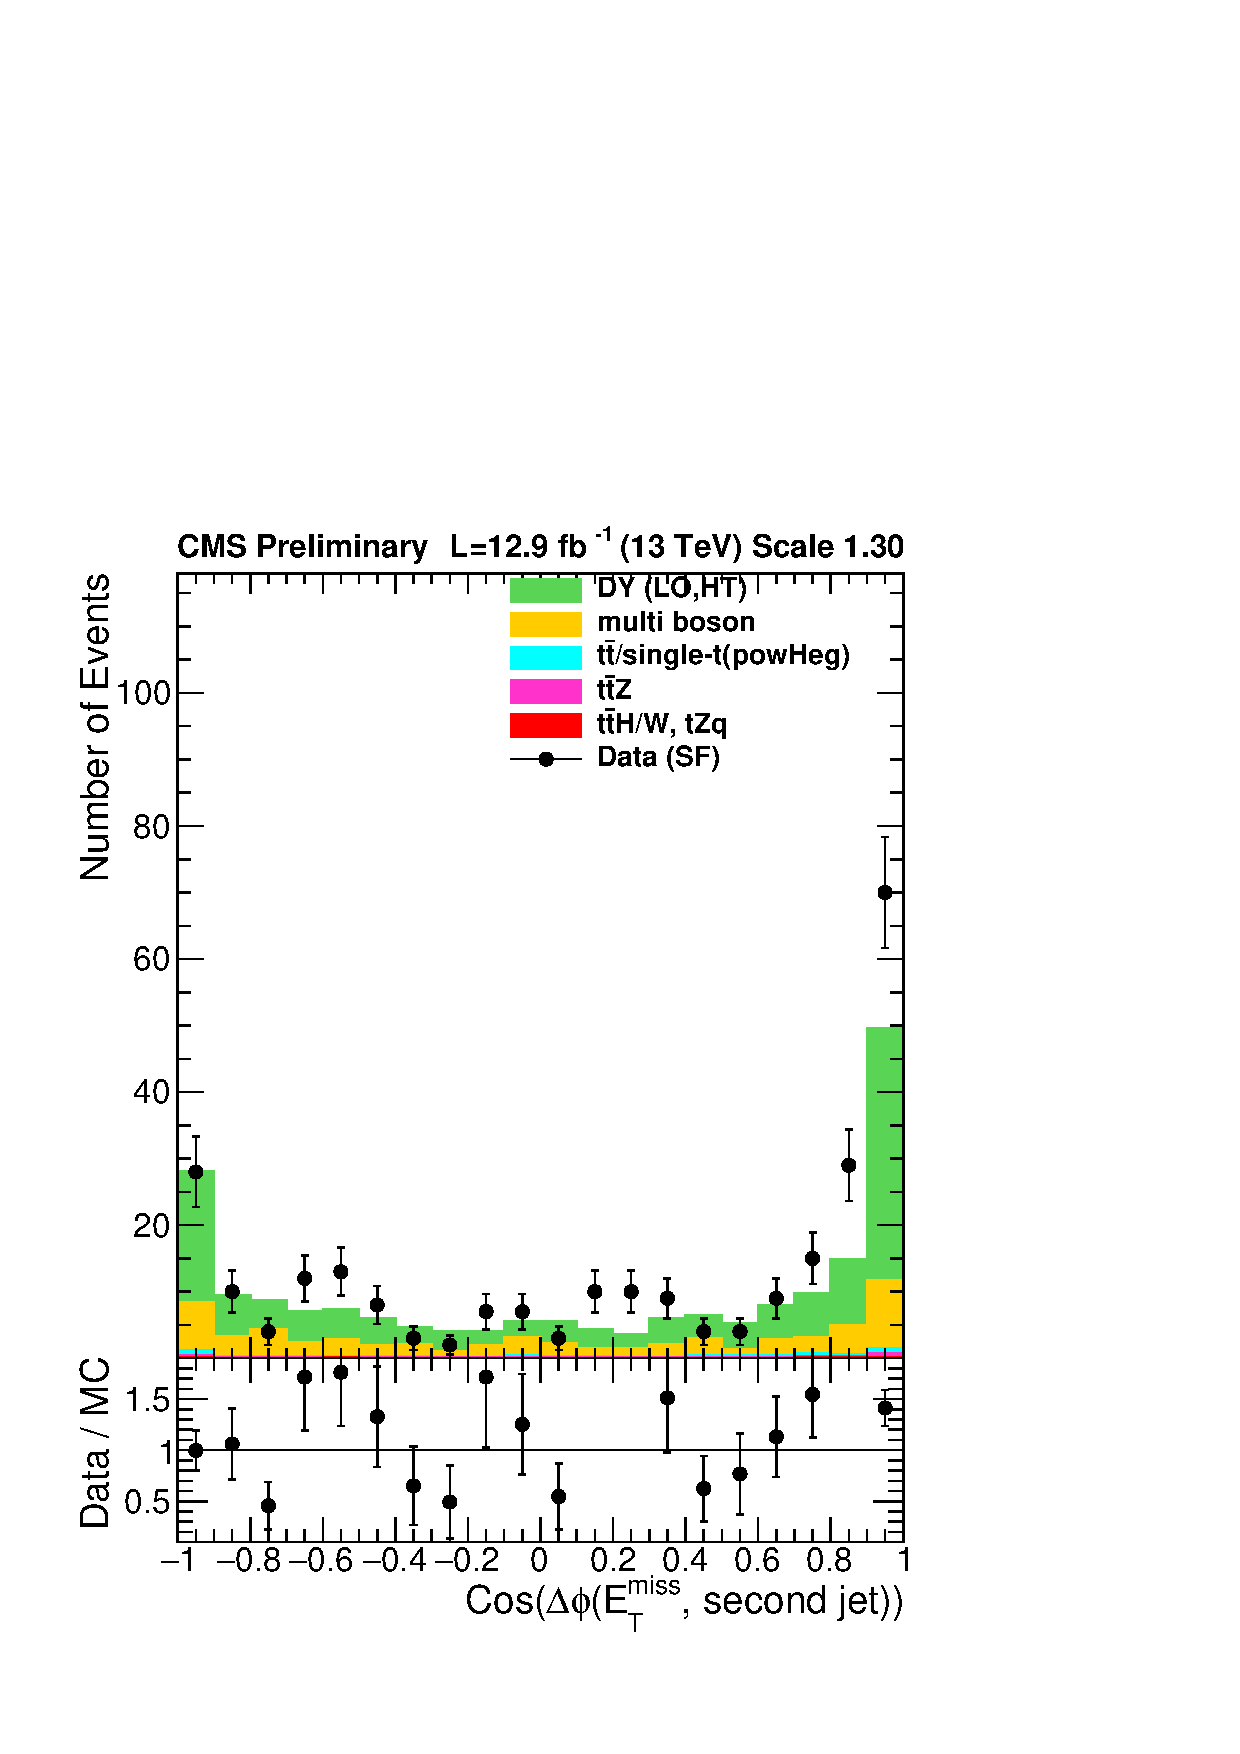
\includegraphics[width=0.4\textwidth]{figures/analysisPlots/SF/njet2-btag0-multiIsoWP-looseLeptonVeto-mll20-onZ-met80-metSig5-mt2ll100/cosMetJet2phi_smallBinning.pdf}}
\caption{Distributions of $\cos{\Delta\phi(\met, \text{jet})}$ for same-flavour ($ee$/$\mu\mu$) events falling within the $Z$-mass window, with two jets and exactly 0 $b$-tags, $\met > 80$ GeV, $S > 5$
     and $\mtll > 100$ GeV.}
\label{fig:DY_afterMetSig}
\end{figure}


\begin{figure}[!hbtp]
\centering
\subfloat[$\cos{\Delta\phi(\met, \text{leading jet})} > 0.8$ or $\cos{\Delta\phi(\met, \text{2nd leading jet})} > \cos{0.25}$][$\cos{\Delta\phi(\met, \text{leading jet})} > 0.8$ or \\ $\cos{\Delta\phi(\met, \text{2nd leading jet})} > \cos{0.25}$]{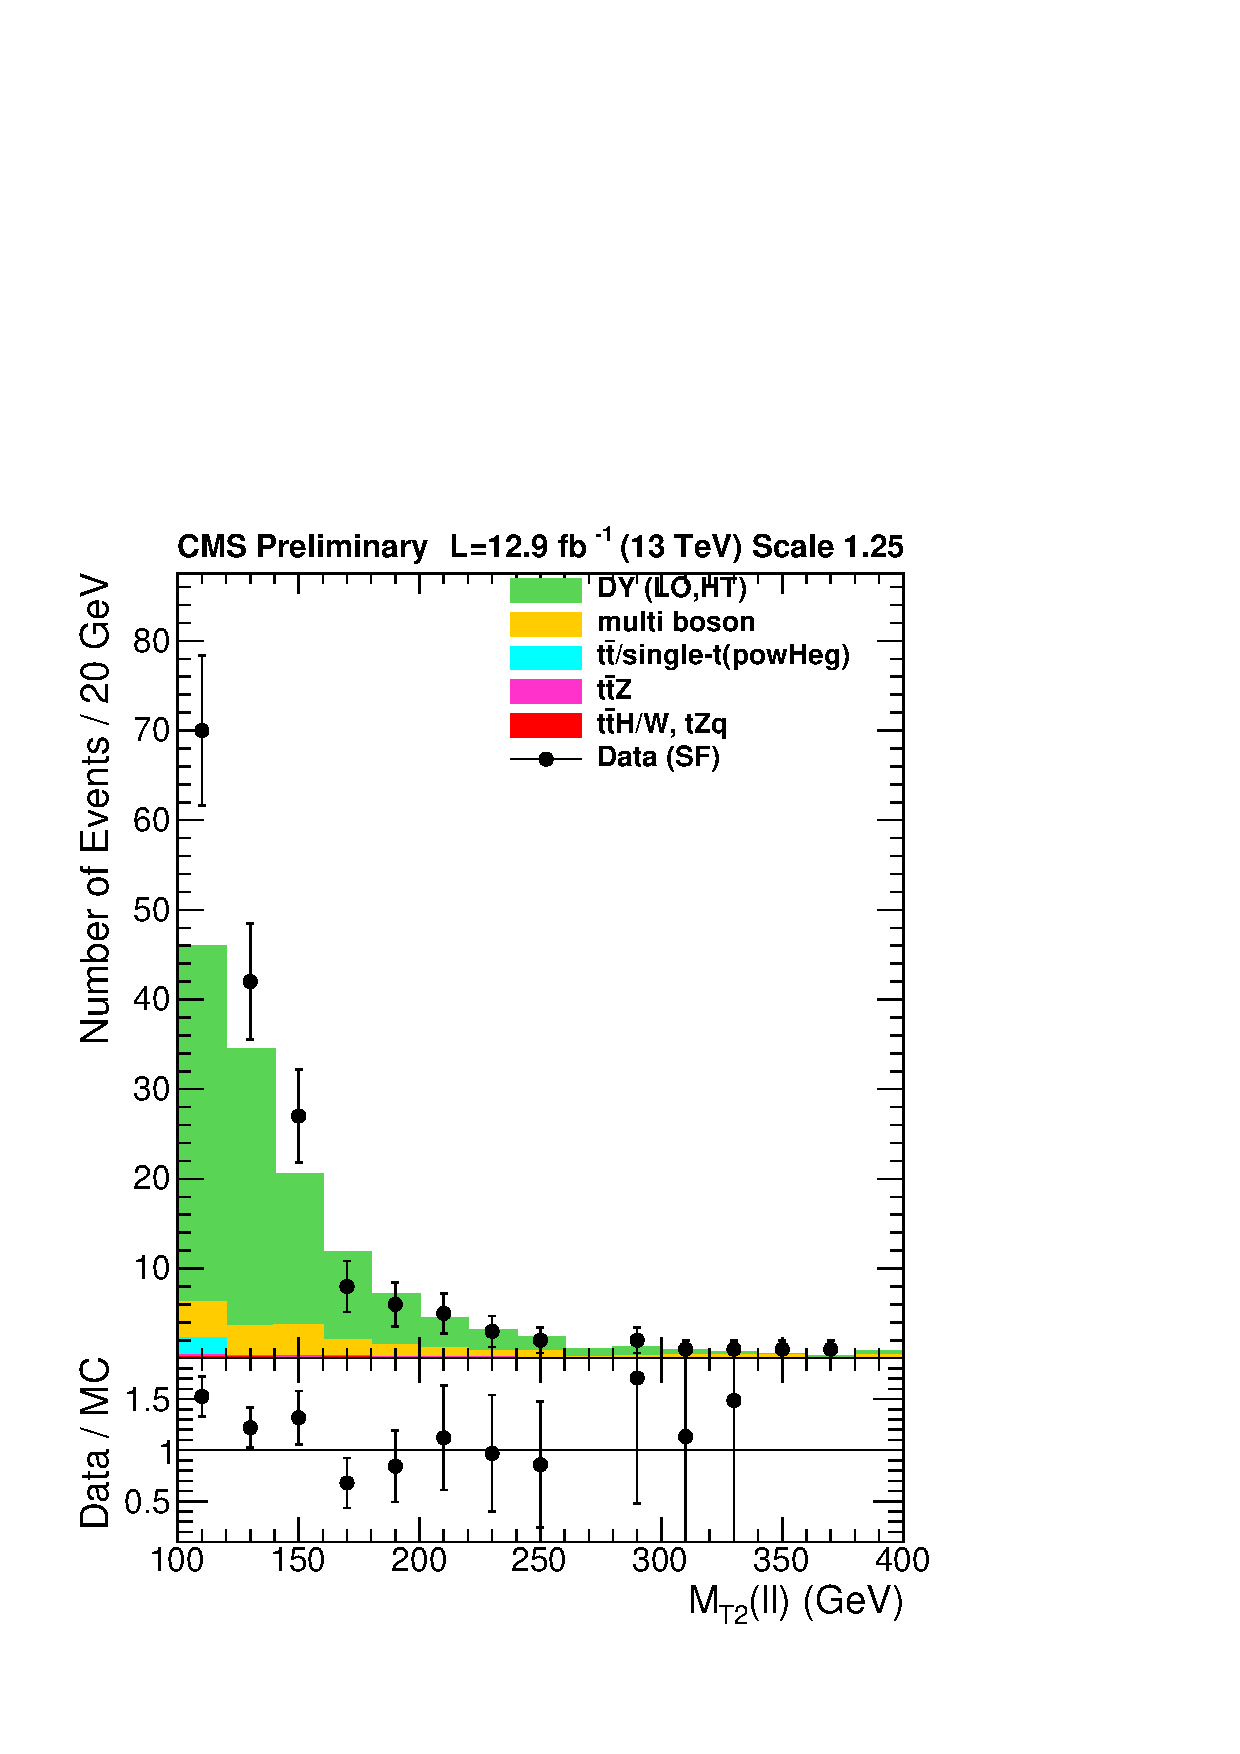
\includegraphics[width=0.4\textwidth]{figures/analysisPlots/SF/njet2-btag0-multiIsoWP-looseLeptonVeto-mll20-onZ-met80-metSig5-dPhiInv-mt2ll100/dl_mt2ll.pdf}}
\subfloat[$\cos{\Delta\phi(\met, \text{leading jet})} < 0.8$ and $\cos{\Delta\phi(\met, \text{2nd leading jet})} < \cos{0.25}$][$\cos{\Delta\phi(\met, \text{leading jet})} < 0.8$ and \\ $\cos{\Delta\phi(\met, \text{2nd leading jet})} < \cos{0.25}$]{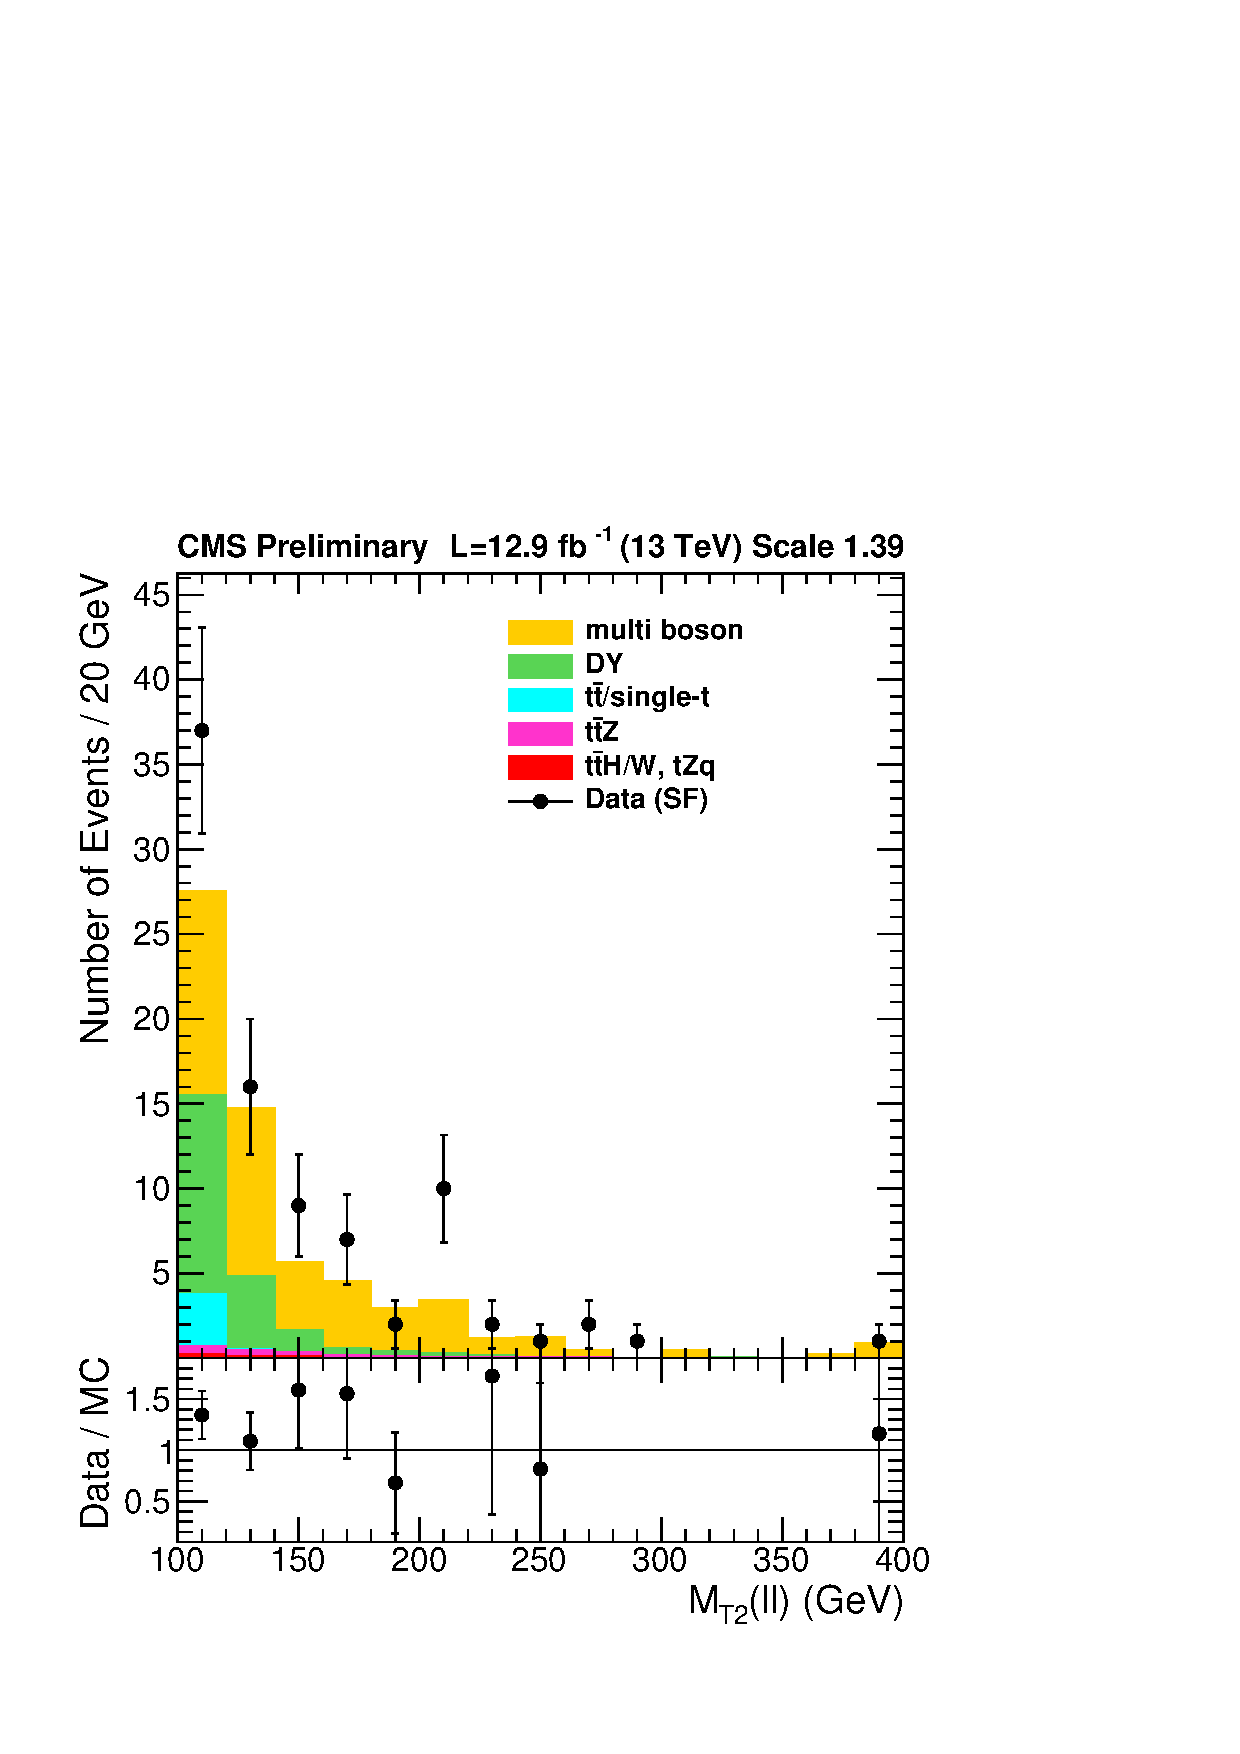
\includegraphics[width=0.4\textwidth]{figures/analysisPlots/SF/njet2-btag0-multiIsoWP-looseLeptonVeto-mll20-onZ-met80-metSig5-dPhiJet0-dPhiJet1-mt2ll100/dl_mt2ll.pdf}}
\caption{Distributions of \mtll in a DY and diboson dominated region for same-flavour ($ee$/$\mu\mu$) events falling within the $Z$-mass window, with two jets and exactly 0 $b$-tags, $\met > 80$ GeV, \metSig $> 5$
     and $\mtll > 100$ GeV.}
\label{fig:DY_dPhiInv}
\end{figure}

\begin{table}
\centering
%\scriptsize
\begin{tabular}{l|ccccccc} 
  selection & DY&TTJets&multiBoson&TTX&observed&DY purity \\ 
  \hline 
  $\met > 50$ GeV & 837.96 & 6.12 & 87.76 & 4.98 & 1052&                                         $89\%$\\ %$1.14\pm0.04$ &
  $\met > 80$ GeV & 261.25 & 5.65 & 64.57 & 3.89 & 392&                                          $77\%$\\ %$1.22\pm0.08$ &
  $\met > 50$ GeV, $\metSig > 5$ & 179.30 & 5.40 & 59.83 & 3.47 & 346&                           $72\%$\\ %$1.55\pm0.11$ &
  $\met > 80$ GeV, $\metSig > 5$ & 132.20 & 5.13 & 57.34 & 3.38 & 257&                           $66\%$\\ %$1.45\pm0.13$ &
  $\met > 50$ GeV, inv. $\Delta\phi$ & 656.29 & 2.38 & 39.14 & 2.26 & 776&                       $94\%$\\ %$1.12\pm0.04$ &
  $\met > 80$ GeV, inv. $\Delta\phi$ & 217.04 & 2.14 & 22.92 & 1.61 & 265&                       $89\%$\\ %$1.10\pm0.08$ &
  $\met > 50$ GeV, $\metSig > 5, \Delta\phi$ & 28.02 & 3.29 & 40.17 & 2.11 & 100&                $37\%$\\ %$1.94\pm0.38$ &
  $\met > 80$ GeV, $\metSig > 5, \Delta\phi$ & 18.45 & 3.14 & 39.49 & 2.07 & 88&                 $29\%$\\ %$2.35\pm0.54$ &
  $\met > 50$ GeV, $\metSig > 5$, inv. $\Delta\phi$ & 151.28 & 2.12 & 19.66 & 1.36 & 246&        $86\%$\\ %$1.47\pm0.11$ &
  $\met > 80$ GeV, $\metSig > 5$, inv. $\Delta\phi$ & 113.75 & 1.99 & 17.85 & 1.31 & 169&        $84\%$\\ %$1.30\pm0.12$ &
\end{tabular} 

\caption{Yields and DY purity in 0b with the listed cuts applied on top of events falling within the $Z$-mass window, having two jets and exactly 0 $b$-tags, and $\mtll > 100$ GeV}
\label{table:scalefactorsDY}
\end{table}

To quantify the robustness of the scale factor we first consider Fig.~\ref{fig:DY_nbtag} which shows a large fraction of DY events without generated (defined as \texttt{hadronFlavour} of $\pm 5$ \cite{twiki:hadronFlavour}) b-quarks entering the $\Nbtags\geq 1$ region. 
The uncertainties on events with only fake b tags are covered by the experimental uncertainties provided by the BTV POG. 
\begin{figure}[!hbtp]
\centering
\subfloat[\Nbtags]{\includegraphics[width=0.45\textwidth]{figures/DY/dy_nbtag.png}}
\caption{Distributions of \Nbtags in simulated DY events in events with and without generated b-quarks.}
\label{fig:DY_nbtag}
\end{figure}
In order to assess the uncertainties on the generated b-quark multiplicity we calculate  the variation of ratios as a function of the {\texttt NNPDF} weights and find a 2\% variation. 
Furthermore, we scale the events with generated b-quarks up and down by 50\% to cover the uncertainty on the modeling of gluon splitting. This translates into an uncertainty~of~25\%~on~$R$. 

In a second step, we invert the requirements on the angular separation of \ETmiss and jets and consequently obtain a region that is dominated by diboson backgrounds as seen in Fig.~\ref{fig:DY_dPhiInv}b.
The purity of diboson backgrounds is approximately 70\%. 
Applying the scale factor $R$ on DY and subtracting again simulated yields from data, we calculate a scale factor of $1.45\pm0.26$ for the diboson background and we add a 25\% uncertainty on the DY component. 
As the DY and diboson scale factors are used to correct the simulation based prediction, their uncertainty is propagated to every signal region in a correlated way.
For completeness, we list the composition of several selections in the on-Z selection with 0 b-tags in Table~\ref{table:scalefactorsDY}. 

%lists the measured scalefactors for different configurations of \met, \metSig and $\Delta\phi(\met, \text{jet})$ cuts. It is not possible to take exactly the same \met cuts
%as in the main analysis, given that very few DY events pass these cuts in combination with the $\mtll > 100 GeV$ requirement. 
%In order to achieve a $\mtll > 100 GeV$ region where DY dominates with sufficient statistics, we need to relax the \met and \metSig cuts and/or invert the $\Delta\phi(\met, \text{jet})$ cuts.
%Given that the region with $\met > 80$ GeV, $\metSig > 5$ and inverted $\Delta\phi$ cuts has a high purity, we choose this as our DY control region.
%Similarly, we derive a scalefactor of $1.45\pm0.26$ for dibosons using the $\met > 80$ GeV, $\metSig > 5$ and $\Delta\phi$ region where dibosons have a purity of 56 \%. While deriving the diboson scalfactors,the DY scalefactor was applied in the subtraction of the residual MC.

\begin{figure}[!hbtp]
\centering
\subfloat[inverted $\Delta\phi$ cuts and $\mtll>100$]{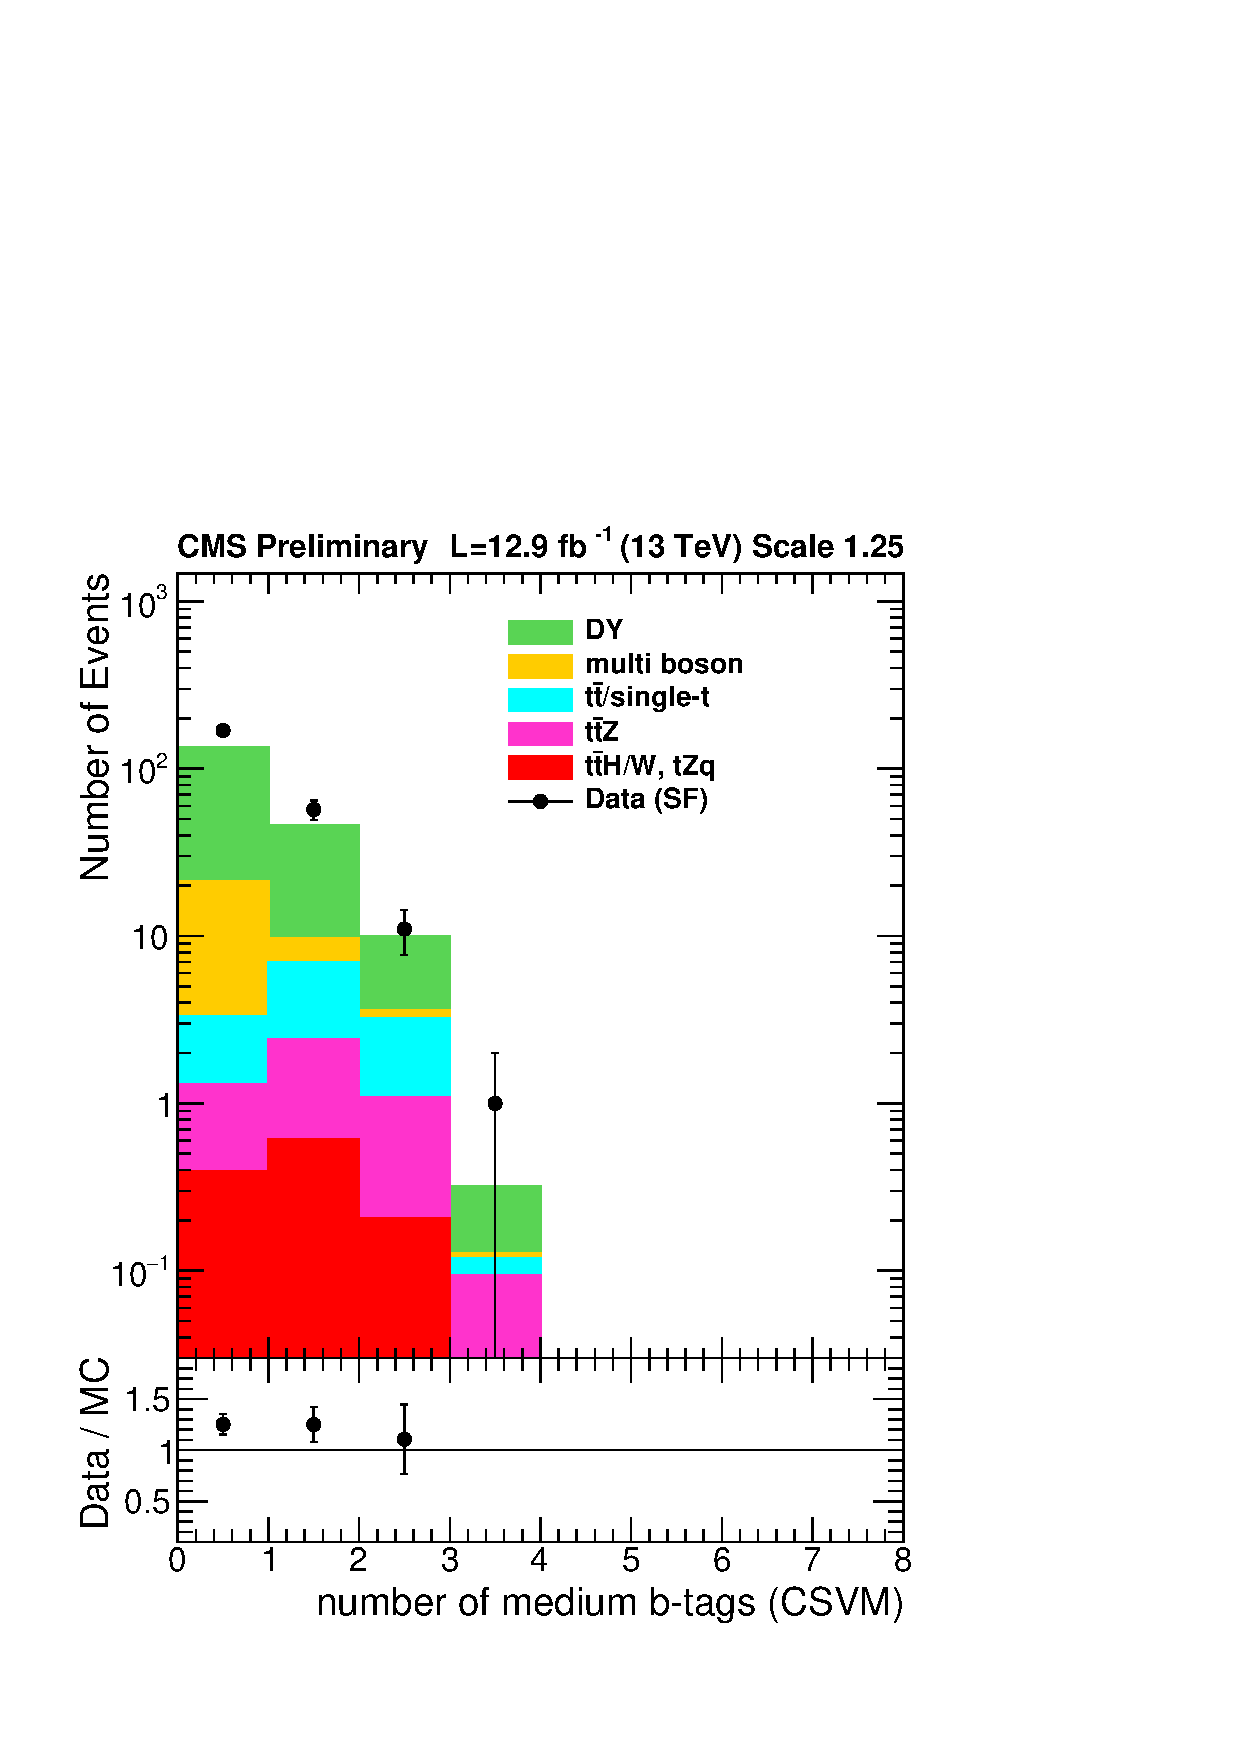
\includegraphics[width=0.45\textwidth]{figures/analysisPlots/SF_log/njet2-multiIsoWP-looseLeptonVeto-mll20-onZ-met80-metSig5-dPhiInv-mt2ll100/nBTag.pdf}}
\subfloat[inclusive]{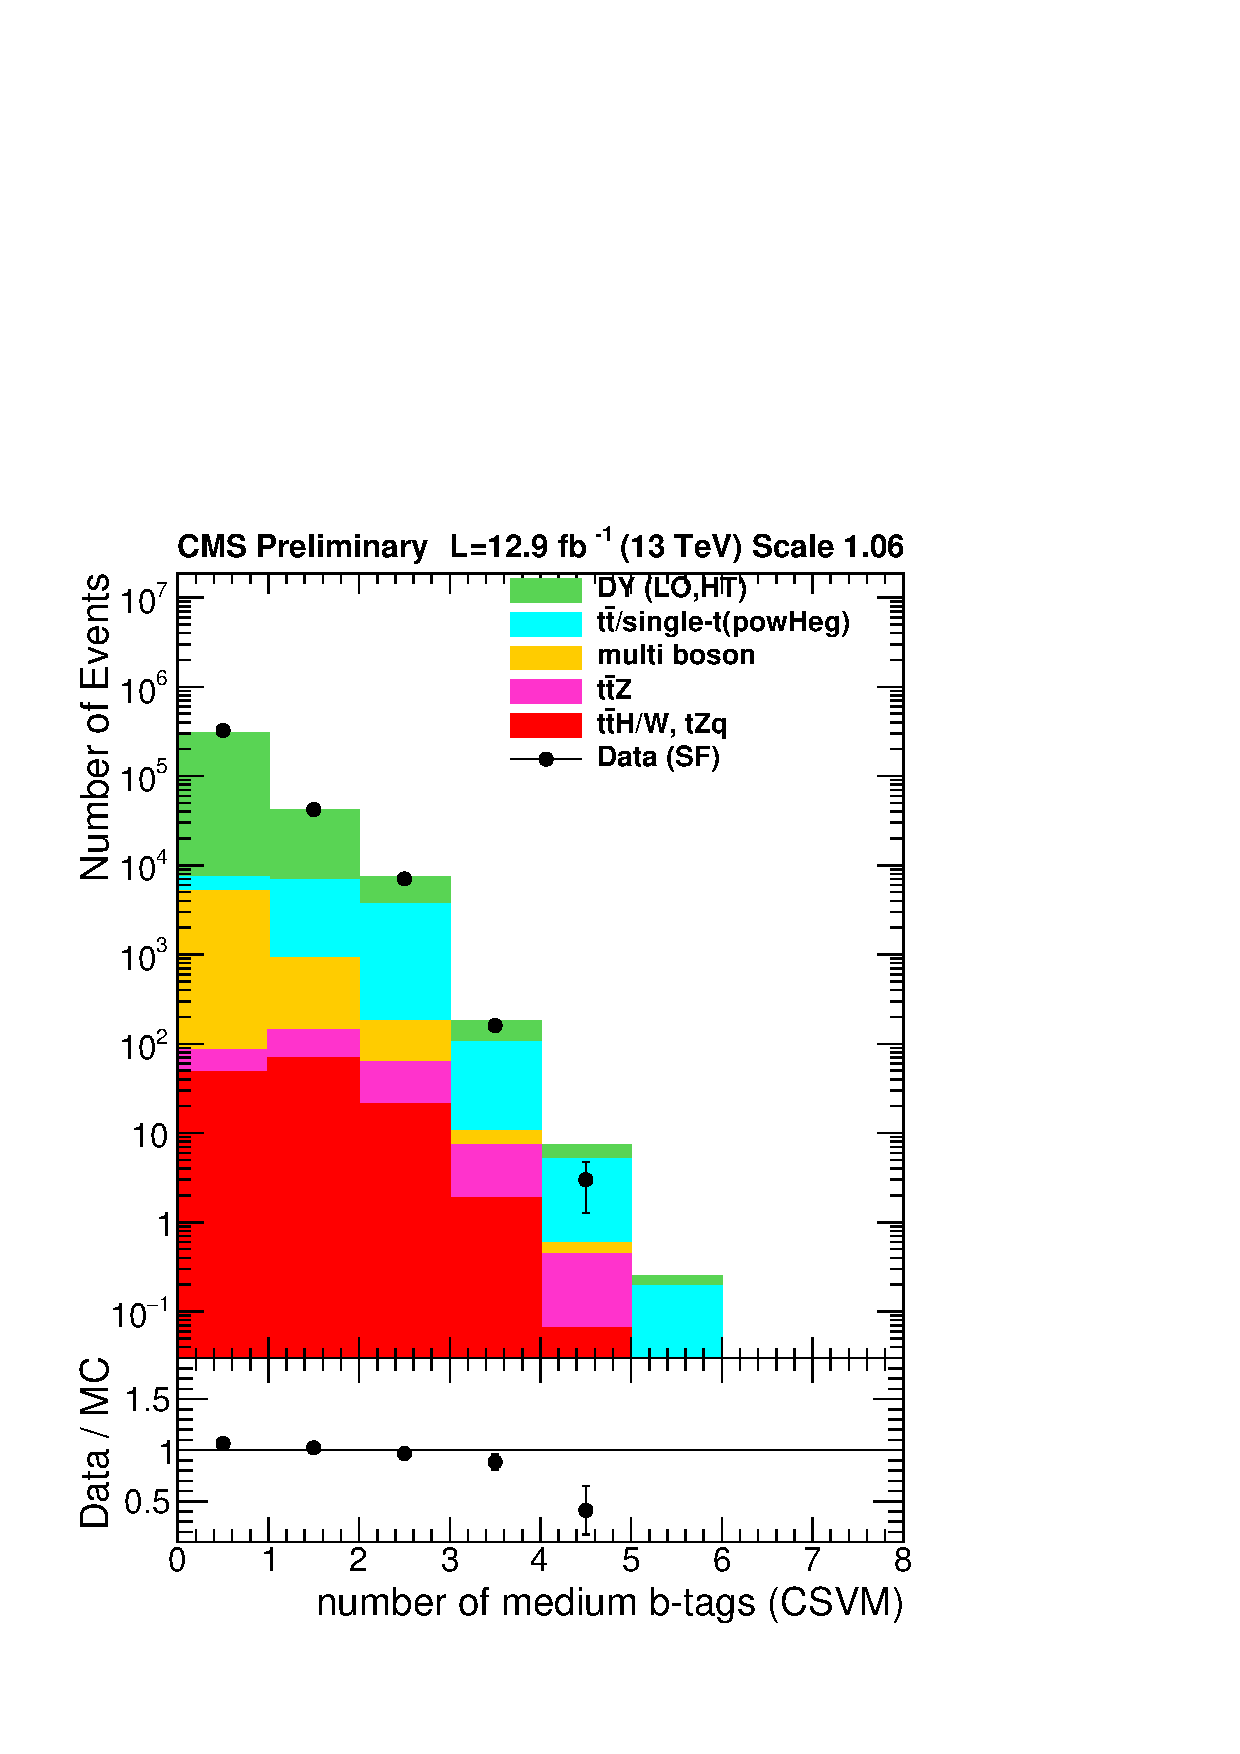
\includegraphics[width=0.45\textwidth]{figures/analysisPlots/SF_log/njet2-multiIsoWP-looseLeptonVeto-mll20-onZ/nBTag.pdf}}
\caption{Data/MC comparison of \Nbtags in the on-Z DY selection with $\mtll>100$~\GeV (left) and, inclusively, when removing the \mtll, \ETmiss, \metSig and $\Delta\phi$ requirements (right).}
\label{fig:DY_nbtag_validation}
\end{figure}

